\chapter{绪\hskip\ccwd{}论}

\section{引言}\label{section 1-1}

随着国民经济和社会的高速发展,以及人们对美好生活的不懈追求,汽车已成为人们日常生活中不可或缺的交通工具之一。据统计,截至2021年底,我国民用汽车保有量高达30151万辆 \cite{gou2022zhong}。然而,汽车数量的急剧增长也给人类社会和自然环境带来了许多挑战。据世卫组织数据,全球每年约有130万人因道路交通事故死亡,另外约有2000至5000万人因事故受到非致命伤害,如致残等 \cite{shi2022dao}。同时,日益严峻的城市交通拥堵问题也给经济发展造成了巨大损失。此外,汽车也是空气污染物排放的主要贡献者之一,仅在2021年,全国汽车污染物排放总量就超过了1401.9万吨 \cite{shen2022zhong}。近年来,随着传感模式、通信技术和计算范式的发展,传统汽车正在向智能化、网联化和协同化方向迅猛发展。以智能网联汽车(Intelligent Connected Vehicle, ICV)为抓手,车联网(Internet of Vehicles, IoV)驱动的智能交通系统(Intelligent Transportation System, ITS)正致力于实现更加安全、高效和可持续发展的下一代交通运输。

近年来,车联网及其推动的智能网联汽车和智能交通系统已上升为我国的重要战略。2019年9月,国务院发布了《交通强国建设纲要》,提出要加强智能网联汽车的研发,通过新基建形成自主可控的车联网核心技术和生态产业链 \cite{zhong2019jiao}。2020年2月,国家发改委等11个部委联合发布了《智能汽车创新发展战略》,明确指出发展智能网联汽车对我国具有重要战略意义,并将突破关键核心技术作为首要战略任务 \cite{guo2020zi}。2022年8月,科技部发文支持建设包括智能港口、智能矿山和自动驾驶在内的十个新一代智能示范应用场景\cite{ke2022ke}。同时,车联网商业化也是业界关注的热点领域。2019年7月,华为发布了首款采用第五代移动通信(The 5th Generation Mobile Communication, 5G)技术的车载通信模组 MH5000,并与一汽、上汽、广汽等18家车企共同成立“5G汽车生态圈”,加速5G技术在汽车产业的商业进程。2020年10月,超过100家包括传统汽车制造商、芯片模组与硬件制造商、地图与定位服务提供商在内的相关企业,在中国上海开展了蜂窝车联网(Cellular-Vehicle-to-Everything, C-V2X)“新四跨”(跨芯片模组、跨终端、跨整车和跨安全平台)应用示范活动。截至2023年2月,已有包括一汽、上汽、广汽、通用、比亚迪和蔚来等十余家车企推出了C-V2X量产车型。

国内外许多一流高校和科研机构围绕车联网、车路协同、无人驾驶、智能交通系统等领域展开了深入探索与研究。清华大学汽车安全与节能国家重点实验室的李克强院士团队在智能网联汽车“中国方案”技术体系的提出和推动方面做出了重要贡献\cite{wang2023design, li2017dynamical, zheng2016stability}。中科院复杂系统管理与控制国家重点实验室的王飞跃院士团队在智能交通的信息物理融合方面取得了显著进展\cite{li2023sharing, liu2021cyber, lv2021guest}。无线移动通信国家重点实验室的陈山枝博士团队致力于C-V2X标准的制定和关键技术的研究,极大推动了车联网的产业化进程\cite{chen2023cellular, chen2020a, chen2017vehicle}。西安电子科技大学综合业务网理论与关键技术国家重点实验室的毛国强教授团队在车联网的高效数据分发、实时感知、ITS应用等方面取得了具有国际影响力的科研成果\cite{zhang2022new, hao2022dhcloc, yue2022towards}。深圳大学Victor C.M Leung 教授团队专注于车联网边缘缓存、任务卸载和资源分配等领域的研究,并取得了系列重要科研成果\cite{sun2023federated, ju2023joint, wang2022efficient}。长安大学赵祥模教授团队在高速公路场景下智能车路协同体系架构以及相关运行安全性与适应性评估技术方面做出了重要贡献\cite{fang2022a, fang2022on, jing2022integrated}。

国际上,加拿大滑铁卢大学Sherman Shen 教授团队在车联网安全\cite{chen2022adaptive}、车路协同\cite{liu2022real}和资源优化\cite{li2022cost}等领域取得了重要的研究突破。瑞典奥斯陆大学Yan Zhang教授团队在车联网边缘计算\cite{dai2022adaptive}、内容缓存\cite{zhang2022digital}和资源分配\cite{sun2022dynamic}等领域做出了突出的贡献。香港理工大学Jiannong Cao 教授团队在车联网边缘计算\cite{yang2022delegating}、计算卸载\cite{dai2023a}和数据分发\cite{yang2020efficient}等领域取得了重要的研究成果。澳大利亚悉尼大学Abbas Jamalipour 教授团队在面向下一代网络中车联网通信\cite{qi2022energy}、感知\cite{iranmanesh2022a}和计算\cite{alam2022multi}等方面取得了重要的研究突破。美国休斯敦大学Zhu Han 教授团队在车联网中安全\cite{khan2023federated}、无线资源分配\cite{zhang2023mean}以及博弈论应用\cite{kang2021joint}等领域展开了深入研究并取得了系列重要成果。加拿大卡尔顿大学F.Richard Yu 教授团队在智能网联汽车中网络安全\cite{alladi2023ambient, liang2023a, bai2022detection}等领域进行了深入研究,并取得了重要的科研成果。香港理工大学Song Guo 教授团队在车联网边缘智能\cite{wang2922imitation, ren2021blockchain, wang2022design}等领域做出了突出贡献。日本东北大学Nei Kato教授团队在车联网中安全\cite{tang2020future}、智能反射面\cite{zhu2022intelligent}和边缘计算\cite{liu2020smart}等领域进行了全面深入的研究,并获得了系列重要科研成果。香港中文大学Guoliang Xing 教授团队在自动驾驶\cite{he2021vi}和信息物理融合系统(Cyber-Physical System, CPS)\cite{shi2022vips}等领域取得了重要研究成果。

2006年,美国国家科学基金会启动了信息物理融合系统研究计划\cite{nfs2006cps},为CPS领域的发展提供了重要支持和契机,自此以后,CPS领域在全球范围内得到了广泛的关注和发展\cite{lee2016introduction}。
2011年,Li等人\cite{li2011human}首次将信息物理融合系统应用于车联网中,车载信息物理融合系统(Vehicular Cyber-Physical System, VCPS)\cite{xia2019zi} 已成为国内外学术界热门的研究领域之一。车载信息物理融合系统利用智能网联汽车的多模态感知能力、车联网通信技术以及端边云的计算、存储和通信资源,形成集智能网联汽车、车联网、边缘计算、云计算等多种技术于一体的综合系统,并实现感知、计算、传输和控制的一体化。然而,车联网具有网络异构高动态、节点资源动态分布、ITS应用需求多元、真实环境复杂等特点,实现车载信息物理融合系统仍然面临巨大挑战。首先,未来车联网是多计算范式、服务架构共存的高动态网络,融合不同范式并最大化其协同效应,在此基础上,融合异质感知信息并评估其质量是 VCPS 的架构基础与驱动核心。其次,车联网中节点资源异构且受限,实现异构资源协同优化以最大化资源利用率是进一步优化 VCPS 服务质量的技术支持。再次,多元化ITS应用对VCPS的质量/开销需求具有差异性,实现VCPS质量-开销均衡是实现高质量低成本可扩展VCPS的理论保障。最后,在动态复杂车联网环境中,设计和实现基于VCPS的典型应用是验证VCPS的必要手段。因此,本文将结合车联网高异构、高动态、分布式特征和智能交通系统的多样化应用需求,从架构融合与质量设计、异构资源协同优化、质量-开销均衡,以及原型系统实现方面进行理论、技术和系统上的综合创新。

\section{研究背景}\label{section 1-2}

本章节将首先介绍车联网的相关概念及其发展历程。接着,以智慧全息路口为例,介绍车载信息物理融合系统,并分析其中所面临的挑战。

\begin{figure}[h]
	\centering
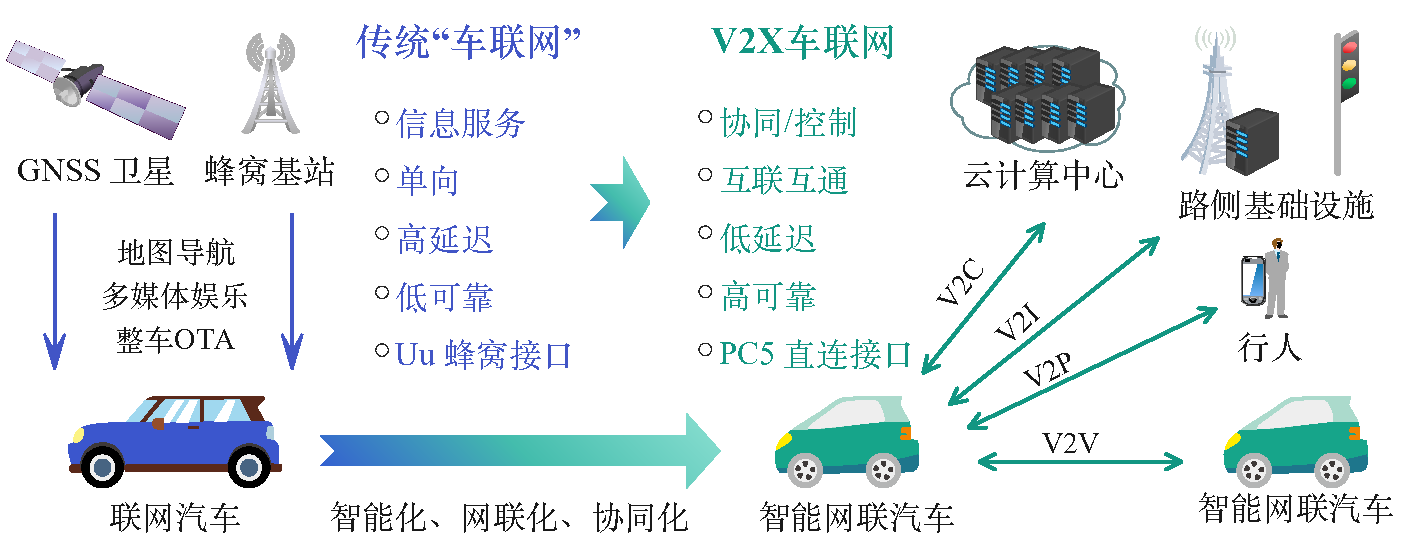
\includegraphics[width=1\columnwidth]{Fig1-1-V2X.pdf}
	\bicaption[车联网演进方向]{车联网演进方向}[Evolution direction of the Internet of Vehicles]{Evolution direction of the Internet of Vehicles}
	\label{fig 1-1}
\end{figure}

车联网是物联网(Internet of Things, IoT)技术在汽车领域的应用形式。早在2G/3G移动网络时代,车联网已应用于利用全球导航卫星系统(Global Navigation Satellite System, GNSS)的定位信息为车辆提供防盗和救援服务。如今,智能网联汽车(如宝马、比亚迪、福特、通用、蔚来以及特斯拉等)都支持空中下载(Over-the-Air, OTA)技术对车机系统进行在线更新。如图 \ref{fig 1-1} 所示,随着汽车朝着智能化、网联化、协同化方向发展,传统的面向信息服务的“车联网”已经转变为与万物互联互通的V2X(Vehicle-to-Everything)车联网。具体而言,V2X车联网是指多种通讯方式的融合,包括车辆间通讯(Vehicle-to-Vehicle, V2V)、车辆与行人通讯(Vehicle-to-Pedestrian, V2P)、车辆与基础设施通讯(Vehicle-to-Infrastructure, V2I)以及车辆与云端通讯(Vehicle-to-Cloud, V2C)。车联网利用实时数据分发,实现人、车、路等交通要素的协同配合,最终实现“聪明的车、智慧的路、协同的云”。此外,车联网还能促进基于单车智能的自动驾驶技术发展,通过车联网通信协助自动驾驶发现潜在危险,提升道路安全。随着我国车联网产业在政策规划、标准体系建设、关键技术研发、应用示范和基础设施建设等多方面的稳步发展,车联网的内涵和外延也在不断发展演进。依托快速落地的新型基础设施建设,车联网不仅广泛服务于智能网联汽车的辅助驾驶、自动驾驶等不同应用,还拓展服务于智慧矿山、智慧港口等企业生产环节以及智慧交通、智慧城市等社会治理领域\cite{zhong2021che}。

\begin{figure}[h]
	\centering
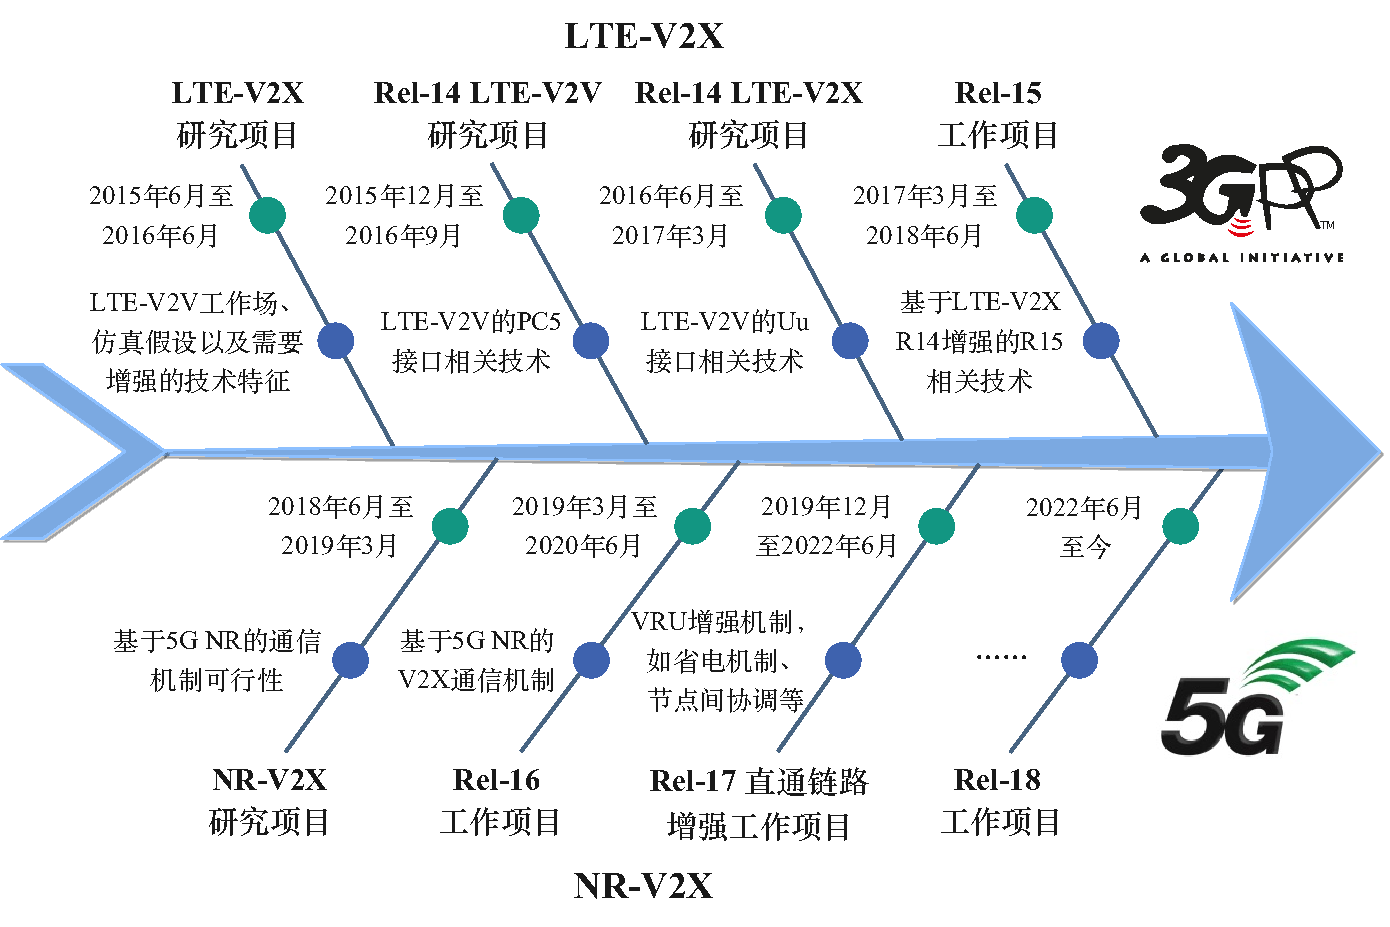
\includegraphics[width=0.95\columnwidth]{Fig1-2-V2X-evolution.pdf}
	\bicaption[3GPP C-V2X 标准演进]{3GPP C-V2X 标准演进}[3GPP C-V2X standard evolution]{3GPP C-V2X standard evolution}
	\label{fig 1-2}
\end{figure}

在车联网通信标准方面,电气和电子工程师协会(Institute of Electrical and Electronics Engineers, IEEE)在2003年提出了专用短距通信技术(Dedicated Short-Range Communication, DSRC)。2010年,IEEE发布了名为无线接入车载环境(Wireless Access in Vehicular Environments, WAVE)的协议栈,其中包括IEEE 802.11p、IEEE 1609.1/.2/.3/.4协议族和SAE J2735消息集字典 \cite{wu2013vehicular}。同时,基于长期演进(Long-Term Evolution, LTE)的V2X通信已形成完善的技术标准体系和产业链\cite{chen2016lte}。此外,IMT-2020(5G)推进组成立了C-V2X工作组,加速基于5G的V2X通信的演进。如图 \ref{fig 1-2} 所示,国际标准组织第三代合作伙伴计划(The 3rd Generation Partnership Project, 3GPP)在2018年启动基于5G新空口(New Radio, NR)的V2X标准研究,并在2020年完成了Rel-16版本的5G NR-V2X标准\cite{saad2021advancements},Rel-17版本进一步优化了功率控制、资源调度等相关技术。5G 汽车协会(5G Automotive Association, 5GAA)、下一代移动通信网络(Next Generation Mobile Network, NGMN)联盟以及5G Americas对IEEE 802.11p和C-V2X进行了技术对比,表\ref{table 1_1}显示C-V2X在传输时延、范围、速率以及可靠性等方面具有显著优势。目前,我国LTE-V2X产业蓬勃发展,与DSRC技术路线之争取得了重大进展。我国已建成基于LTE-V2X技术的完备产业链,芯片、模组、车载终端(Onboard Unit, OBU)、路侧设备(Roadside Unit, RSU)等均已成熟且经过了“三跨”“四跨”“新四跨”以及大规模测试,满足了商用部署条件。

\begin{table}[h]\small
\setstretch{1.245} %设置具有指定弹力的橡皮长度(原行宽的1.2倍)
\centering
\bicaption[C-V2X和IEEE 802.11p技术对比]{C-V2X和IEEE 802.11p技术对比\cite{cheng2021feng}}[Technical comparisons of C-V2X and IEEE 802.11p]{Technical comparisons of C-V2X and IEEE 802.11p \cite{cheng2021feng}}
\label{table 1_1}
\resizebox{\columnwidth}{!}{%
\begin{tabular}{@{}ccccc@{}}
\toprule
\begin{tabular}[c]{@{}c@{}}C-V2X\\ 技术优势\end{tabular} &
 \begin{tabular}[c]{@{}c@{}}具体技术\\ 或性能\end{tabular} &
IEEE 802.11p &
\begin{tabular}[c]{@{}c@{}}LTE-V2X\\ (3GPP R14/R15)\end{tabular} &
\begin{tabular}[c]{@{}c@{}}NR-V2X\\ (3GPP R16)\end{tabular} \\ \midrule
低时延 &
  时延 &
  不确定时延 &
  \begin{tabular}[c]{@{}c@{}}R14: 20ms\\ R15: 10ms\end{tabular} &
  3ms \\ 
\begin{tabular}[c]{@{}c@{}}低时延/\\ 高可靠\end{tabular} &
  \begin{tabular}[c]{@{}c@{}}资源分配\\ 机制\end{tabular} &
  CSMA/CA &
  \begin{tabular}[c]{@{}c@{}}支持感知+半持续\\ 调度和动态调度\end{tabular} &
  \begin{tabular}[c]{@{}c@{}}支持感知+半持续\\ 调度和动态调度\end{tabular} \\ 
\multirow{3}{*}[3.4ex]{高可靠} &
  可靠性 &
  不保证可靠性 &
  \begin{tabular}[c]{@{}c@{}}R14: \textgreater{}90\%\\ R15: \textgreater{}95\%\end{tabular} &
  支持99.999\% \\  
 &
  信道编码 &
  卷积码 &
  Turbo &
  LDPC \\ 
 &
  重传机制 &
  不支持 &
  \begin{tabular}[c]{@{}c@{}}支持HARQ,\\ 固定2次传输\end{tabular} &
  \begin{tabular}[c]{@{}c@{}}支持HARQ,\\ 传输次数灵活,\\ 最大支持32次传输\end{tabular} \\ 
\multirow{2}{*}[0ex]{\begin{tabular}[c]{@{}c@{}}更远传输\\ 范围\end{tabular}} &
  通信范围 &
  100m &
  \begin{tabular}[c]{@{}c@{}}R14: 320m\\ R15: 500m\end{tabular} &
  1000m \\  
 &
  波形 &
  OFDM &
  \begin{tabular}[c]{@{}c@{}}单载波频分复用\\ (SC-FDM)\end{tabular} &
  循环前缀(CP)-OFDM \\ 
\multirow{2}{*}[1.5ex]{\begin{tabular}[c]{@{}c@{}}更高传输\\ 速率\end{tabular}} &
  \begin{tabular}[c]{@{}c@{}}数据传输\\ 速率\end{tabular} &
  典型6Mbit/s &
  \begin{tabular}[c]{@{}c@{}}R14: 约30Mbit/s\\ R15: 约300Mbit/s\end{tabular} &
  \begin{tabular}[c]{@{}c@{}}与带宽有关,40MHz\\ 时R16单载波2层数据\\ 传输支持约400Mbit/s,\\ 多载波情况下更高\end{tabular} \\ 
 &
  调制方式 &
  64QAM &
  64QAM &
  256QAM \\ \bottomrule
\end{tabular}%
}
\end{table}

\begin{figure}[h] 
	\centering
	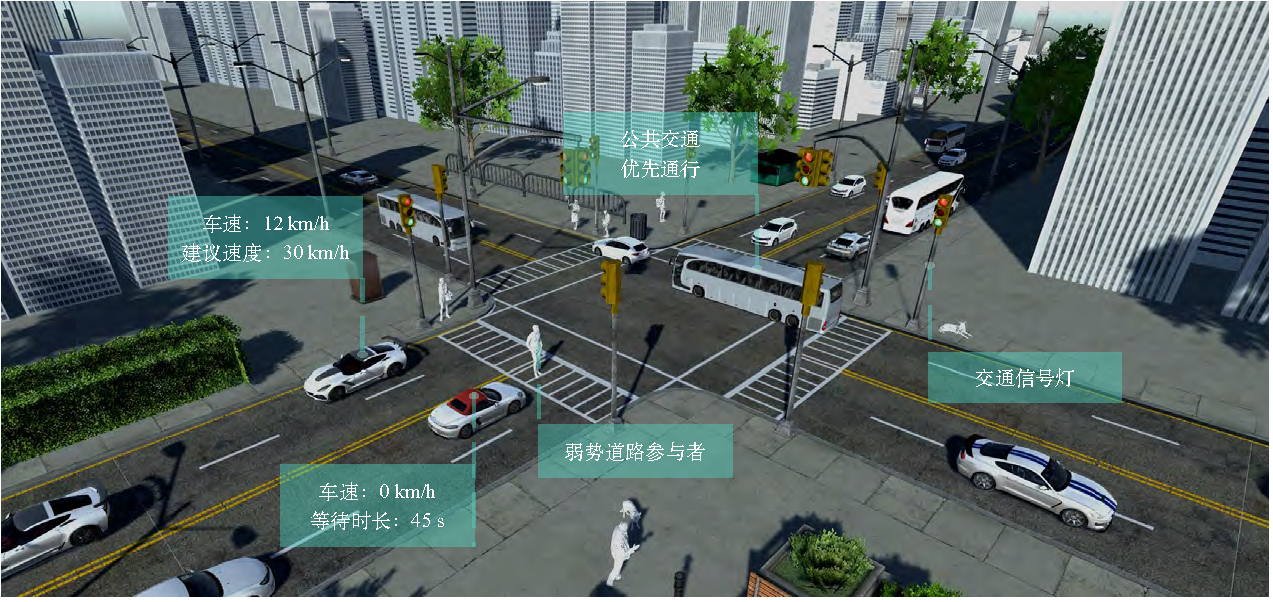
\includegraphics[width=1\columnwidth]{Fig1-3-intersection.pdf}
	\bicaption[基于车载信息物理融合的智慧全息路口]{基于车载信息物理融合的智慧全息路口}[Intelligent holographic intersection based vehicular cyber-physical fusion]{Intelligent holographic intersection based vehicular cyber-physical fusion}
	\label{fig 1-3}
\end{figure}

如图 \ref{fig 1-3} 所示,智慧全息路口是基于车载信息物理融合技术的智慧交通管理系统。它通过将城市道路上的全要素进行数字化还原,为各类智能交通系统应用提供数据支撑。智慧全息路口利用道路基础设施和智能网联汽车上搭载的激光雷达、毫米波雷达、摄像头等多源传感设备,对路口进行全方位感知和全要素采集。通过传感设备实时感知交通流量、车速、车道变化等数据,并结合高精度地图呈现路口数字化上帝视角,精准刻画路口上的每一条车道、每一个交通信息灯的状态,以及每一辆车的行为轨迹。在实现路口全要素数字化还原的过程中,采用车载边缘计算技术将异构感知数据在边缘节点进行融合处理,从而提高数据处理速度,降低数据传输成本。同时,利用目标检测、目标跟踪、行为分析等算法对感知数据进行预处理,进一步提高数据准确性和精度,为后续的交通管理、交通安全和交通规划等应用提供更可靠的数据基础。

智慧全息路口不仅可以实现路口全要素数字化还原,而且可以进一步作为车载信息物理融合系统的外在展示和数据内核,支撑各种智能交通系统的应用。例如,全息路口可以为公交优先通行、绿波通行、弱势道路参与者(Vulnerable Road User, VRU)感知等 ITS 应用提供强有力的支持。在公交优先通行方面,全息路口可以根据公交车的实时位置和行驶速度,并结合路口的交通状况,提前调整信号控制策略,使公交车获得更好的通行效率和服务。在绿波通行方面,全息路口可以通过感知路口的交通流量和车速等信息,实现路口绿灯时长的自适应调整,从而实现车辆在绿波通信路段上的高效通行。在 VRU 感知方面,全息路口可以利用摄像头等传感设备或V2P通信感知VRU(如行人、自行车、残疾人等)的存在和行动轨迹,提供实时的路口状态信息和预警信息,保障弱势道路参与者的通行便利和交通安全。

通过以上讨论可知,车载信息物理融合系统是实现各类ITS应用的基础。然而,在高异构、高动态、分布式的车联网中,实现车载信息物理融合系统以满足多元ITS应用需求仍然面临着诸多问题和挑战。因此,针对以上问题和挑战,需要进一步展开全面深入的研究。具体地,首先,异构车联网亟需服务架构融合创新,并设计车载信息物理融合质量指标。未来车联网是多服务范式并存的高异构移动网络,因此需要研究异构车联网融合服务架构,以最大化不同服务范式的协同效应,并支持VCPS的部署实现。同时,现有研究都没有对VCPS进行整体深入的评估。因此,需要设计基于多源异质感知信息融合的VCPS质量指标,并通过控制车辆感知行为与资源分配提升VCPS系统质量。其次,异构资源亟需协同优化。车联网中的通信和计算资源分布在不同的车辆和基础设施中,因此需要针对异构资源进行协同优化,支持VCPS中计算任务分布式处理,以进一步提升系统服务质量。再次,车载信息物理融合系统亟需质量-开销均衡优化。车载信息物理融合系统需要在保证实时性和准确性的同时,考虑资源开销和能耗问题。因此,需要研究质量-开销均衡的优化策略,以提高系统的资源利用率的同时降低能耗。最后,亟需实现原型系统以验证VCPS性能。通过在真实车联网环境中搭建原型系统,可以进一步验证车载信息物理融合系统的可行性和有效性,为其在实际应用中提供更可靠的支持和保障。

\section{国内外研究现状}\label{section 1-3}

车载信息物理融合系统是实现各类智能交通系统应用的基础,其已成为国内外学术界研究的热点之一。本章节将对国内外相关研究工作进行梳理和总结,并从以下几个方面进行详细阐述:

\subsection{车联网服务架构研究与现状}

随着智能交通系统应用的不断涌现,传统车联网架构已无法满足大规模、高可靠、低时延的需求,因此研究人员正致力于将软件定义网络(Software Defined Network, SDN)新范式应用于车联网中。SDN通过分离数据平面和控制平面,实现了高度灵活的数据调度策略和网络功能虚拟化(Network Functions Virtualization, NFV)。Liu等人\cite{liu2016cooperative}首次将SDN概念应用于车联网中,提出了软件定义车联网(Software Defined Vehicular Network, SDVN),并在此基础上提出了基于混合V2I/V2V通信的在线协同数据调度算法,以提高数据分发的性能。Dai等人\cite{dai2018cooperative}设计了基于SDN的异构车联网中具有时间约束的时态信息服务调度方案。Luo等人\cite{luo2018sdnmac}提出了基于SDN的媒体接入(Media Access Control, MAC)协议以提高车联网的通信性能。Liu等人\cite{liu2018coding}提出了基于SDN的服务架构,并结合车辆缓存和网络编码来提高带宽利用率。Zhang等人\cite{zhang2022ac-sdvn}设计了解决SDVN中视频组播安全问题的安全访问控制协议,实现了多播视频请求车辆和RSU的身份认证。Zhao等人\cite{zhao2022elite}提出了基于智能数字孪生技术的软件定义车联网分层路由方案,克服了SDVN架构中高动态拓扑局限性。Lin等人\cite{lin2023alps}研究了基于SDVN的自适应链路状态感知方案,能够在信标间隔内及时获取链路状态信息,减少数据包丢失。Ahmed等人\cite{ahmed2023deep}提出了基于SDVN中车辆传感器负载均衡算法,并提出了数据包级入侵检测模型,可以跟踪并有效识别网络攻击。然而,现有大部分工作都仅是从数据分发、路由缓存、网络安全等方面展开了研究,缺乏对整体架构的深入分析。

移动边缘计算(Mobile Edge Computing, MEC)\cite{mao2017a}通过将计算、存储和网络资源靠近移动终端设备,提供更快速、更可靠的服务,同时减少网络流量消耗和服务延迟。越来越多的研究考虑将MEC范式应用在车联网环境中以提高系统实时性、可靠性和安全性。Liu等人\cite{liu2017a}首次将移动边缘计算融入车联网中,提出了车载边缘计算(Vehicular Edge Computing, VEC),并集成了不同类型的接入技术,以提供低延迟和高可靠性的通信。Lang等人\cite{lang2022cooperative}设计了基于区块链技术的协同计算卸载方案,以提高VEC资源的利用效率,并确保计算卸载的安全性。Liu等人\cite{liu2021fog}研究了端边云协同架构中的合作数据传播问题,并提出了基于Clique的算法来联合调度网络编码和数据分发。Dai等人\cite{dai2021edge}设计了基于自适应比特率多媒体流的VEC架构,其中边缘节点给以不同质量等级编码的文件块提供缓存和传输服务。Zhang等人\cite{zhang2022digital}提出了车载边缘缓存技术,动态调整边缘节点和车辆的缓存能力以提高服务的可用性。Liu等人\cite{liu2020adaptive}提出了两层VEC架构,利用云、静态边缘节点和移动边缘节点来处理时延敏感性任务。Liao等人\cite{liao2021learning}研究了空地一体的VEC任务卸载策略,其中车辆能够学习具有多维意图的长期策略。Liu等人\cite{liu2023mobility}提出了利用车辆计算资源来提高VEC场景下任务执行效率的计算任务卸载方案。Liu等人\cite{liu2023asynchronous}研究了VEC中任务卸载和资源管理的联合优化问题,并采用异步深度强化学习算法来寻找最优解。然而,上述研究缺乏考虑异构车联网中不同服务架构的协同效应。

\subsection{车载信息物理融合系统质量指标研究与现状}

越来越多的研究人员聚焦于车载信息物理融合系统的预测、调度和控制技术,旨在有效提高 VCPS 系统的整体性能和可靠性。在预测技术方面,Zhang等人 \cite{zhang2021a} 提出了基于 VCPS 架构的车辆速度曲线预测方法,其协同 VCPS 中的不同控制单元来完成速度曲线预测。Albaba等人 \cite{albaba2021driver} 则结合深度Q网络(DQN)和层次博弈论,对高速公路驾驶场景中的驾驶员行为进行预测,其中k级推理被用来模拟驾驶员的决策过程。Zhang等人 \cite{zhang2020data} 提出了变道行为预测模型和加速预测模型。在此基础上,对车辆状态进行预测,并通过动态路由算法实现车辆之间的协同合作,以优化资源利用率和降低能源消耗。Zhou等人 \cite{zhou2021wide} 提出了基于宽-注意力和深度-组合模型用于交通流量预测。其中,宽-注意力模块和深度-组合模块分别用于提取全局关键特征和推广局部关键特征。在调度技术方面,Li等人 \cite{li2020cyber} 考虑了车辆移动性,并开发了基于物理比率-K干扰模型的广播方案,以确保通信的可靠性。Lian等人 \cite{lian2021cyber} 提出了基于既定地图模型路径规划的调度方法,以优化路径利用效率。在控制技术方面,Hu等人 \cite{hu2017cyber} 提出了燃油最优控制器,基于车队头车状态优化车辆速度和无级变速箱齿轮比。Dai等人 \cite{dai2016a} 提出了自主交叉路口控制机制,以确定车辆通过交叉路口的优先权。Lv等人 \cite{lv2018driving} 提出了用于三种典型驾驶方式下控制车辆加速的自适应算法。上述研究集中于支持 VCPS 的不同技术,如轨迹预测、路径调度和车辆控制等,虽然促进了各种 ITS 应用的实施,但是均建立在车联网中高质量物理元素建模信息可用的假设基础上,并未对车载信息物理融合质量进行定量分析。

部分研究工作侧重于利用深度强化学习(Deep Reinforcement Learning, DRL)优化 VCPS 中车辆感知和信息融合。Dong等人 \cite{dong2020spatio} 提出了基于 DQN 的方法,融合本地环境信息并实现可靠的车道变更决策。Zhao等人 \cite{zhao2020social} 设计了基于近似策略优化(Proximal Policy Optimization, PPO)的社会意识激励机制,以得出最佳的长期车辆感知策略。Mika等人 \cite{mlika2022deep} 提出了基于深度确定性策略梯度(Deep Deterministic Policy Gradient, DDPG)的解决方案,通过调度资源块和广播覆盖来优化信息时效性。然而,上述算法不能直接应用于 VCPS 中的协同感知和异构信息融合,并且,当考虑到多辆车场景时,上述算法并不适用。另一方面,部分研究对 VCPS 中的信息质量进行了评估。Liu等人 \cite{liu2014temporal} 提出了用于 VCPS 中时态数据传播的调度算法,其在实时数据传播和及时信息感知之间取得了平衡。Dai等人 \cite{dai2019temporal} 提出了进化多目标算法,以提高信息质量和改善数据到达率。Liu等人 \cite{liu2014scheduling} 提出了两种在线算法,通过分析传播特性来调度不同一致性要求下的时态数据传播。Rager等人 \cite{rager2017scalability} 开发了刻画真实网络随机性的框架,对随机数据负载进行建模以提高信息质量。Yoon等人 \cite{yoon2021performance} 提出了车联网合作感知框架,考虑到通信损耗和车辆随机运动,以获得车辆的精确运动状态。上述研究主要聚焦于 VCPS 中数据及时性、准确性或一致性方面的信息质量评估。然而,这些研究仅考虑了同质数据项层面的质量评估,没有针对车载信息物理融合进行质量评估。

\subsection{车联网资源分配与任务卸载研究与现状}

车联网中的资源分配一直是学术界的研究热点 \cite{noor-a-rahim2022a},大量研究人员针对车联网中通信资源分配进行了深入研究。He等人 \cite{he2022meta} 设计了动态车联网资源管理框架,其采用马尔可夫决策过程(Markov Decision Process, MDP)和分层强化学习相结合的方法,可以显著提高资源管理性能。Lu等人 \cite{lu2021user} 提出了基于用户行为的虚拟网络资源管理方法,以进一步优化车联网通信。Peng等人 \cite{peng2020deep} 提出了车联网资源管理方案,通过应用 DDPG 方法解决了多维资源优化问题,实现了资源快速分配,并满足了车联网服务质量(Quality of Service, QoS)要求。Wei等人 \cite{wei2022multi} 针对车联网云计算中的资源分配问题,从提供者和用户双重视角出发,提出了改进的 NSGA-II 算法来实现多目标优化。Peng等人 \cite{peng2021multi} 研究了无人机辅助车联网中的多维资源管理问题,并提出了基于多智能体深度确定性策略梯度(Multi-Agent Deep Deterministic Policy Gradient, MADDPG)的分布式优化方法,实现了车辆资源联合分配。为了进一步提高频谱利用率和支持更多车辆接入,部分研究将非正交多址接入(Non-Orthogonal Multiple Access, NOMA)技术融入车联网中。Patel等人 \cite{patel2021performance} 评估了基于 NOMA 的车联网通信容量,其数值结果显示,NOMA 通信容量比传统的正交多址接入(Orthogonal Multiple Access, OMA)高出约20\%。Zhang等人 \cite{zhang2021centralized} 利用基于图的匹配方法和非合作博弈(Non-Cooperative Game, NCG)分布式功率控制,为NOMA车联网开发了集中式两阶段资源分配策略。Zhu等人 \cite{zhu2021decentralized} 考虑随机任务到达和信道波动,提出了最优功率分配策略,以最大化长期的功率消耗和延迟。Liu等人 \cite{liu2019energy} 在基于 NOMA 的车联网中,提出了基于交替方向乘子法(Alternating Direction Method of Multipliers, ADMM)的功率分配算法。然而,上述研究主要是基于单边缘节点的情况,无法处理不同边缘节点之间的相互干扰情况。因此,仍然需要探索更加复杂的多边缘节点环境下的资源分配策略,以提高车联网的性能和可靠性。


随着车载边缘计算的发展,大量研究专注于 VEC 中的任务卸载和资源分配。其中,Liu等人\cite{liu2021rtds}提出了多周期任务卸载的实时分布式方法,通过评估 VEC 中的移动性感知通信模型、资源感知计算模型和截止时间感知奖励模型。Shang等人\cite{shang2021deep}研究了节能的任务卸载,并开发了基于深度学习的算法来最小化能耗。为了最小化执行延迟、能源消耗和支付成本的加权和,Liu等人\cite{liu2022a}提出了结合 ADMM 和粒子群优化(Particle Swarm Optimization, PSO)的任务卸载算法。Chen等人\cite{chen2020robust}设计了带有故障恢复功能的计算卸载方法,以减少能源消耗并缩短服务时间。为了实现超高可靠低时延通信(ultra-Reliable and Low-Latency Communication, uRLLC)服务需求下最大化吞吐量,Pan等人\cite{pan2022asynchronous}提出了基于异步联合 DRL 的计算卸载方案。Zhu等人\cite{zhu2022a}提出了用于智能反射面(Intelligent Reflecting Surface, IRS) 辅助下的 VEC 的动态任务调度算法,优化有限资源分配并考虑了车辆的移动模式、传输条件和任务大小以及并发传输之间的相互干扰。此外,部分研究聚焦于采用多智能体强化学习(Multi-Agent Deep Reinforcement Learning, MADRL)算法的任务卸载和资源分配。Alam等人\cite{alam2022multi}开发了基于 DRL 的多智能体匈牙利算法,用于 VEC 中的动态任务卸载以满足延迟、能耗和支付费用需求。Zhang等人\cite{zhang2021adaptive}提出了基于 MADDPG 的边缘资源分配方法,在严格延迟约束下最小化车辆任务卸载成本。为了同时满足严格延迟要求和最小带宽消耗,He等人\cite{he2021efficient}提出了用于车辆带宽分配的多智能体行动者-评论家(Multi-Agent Actor-Critic, MAAC)算法。然而,以上研究工作都没有考虑实时任务卸载和通信/计算资源分配的协同优化。

部分研究专注于VEC的联合通信和计算资源分配。Cui等人\cite{cui2021reinforcement}提出了多目标强化学习方法,通过协同通信和计算资源的分配来减少系统延迟。Han等人\cite{han2020reliability}设计了基于动态规划(Dynamic Programming, DP)的资源分配方法,实现了耦合车辆通信和计算资源的可靠性计算。Xu等人\cite{xu2021socially}采用契约理论为每个潜在的内容供应商和内容请求者分配通信和计算资源。少数研究者研究了联合任务卸载和资源分配。Dai等人\cite{dai2021asynchronous}提出了异步的DRL算法,实现了异构服务器数据驱动的任务卸载。此外,Dai等人 \cite{dai2022a}开发了概率计算卸载方法,根据边缘节点的计算分配概率进行计算卸载的独立调度。Nie等人\cite{nie2021semi}提出了在无人机辅助VEC中基于MADRL算法的联合优化资源分配和功率控制策略。然而,现有研究主要基于集中式调度,通信开销和调度复杂性较高,不适用于大规模的车联网。

\subsection{车载信息物理融合中质量/开销优化研究与现状}

近年来,许多研究人员致力于提高车载信息物理融合中的 QoS,以提升 ITS 应用的用户体验。其中,Wang等人\cite{wang2016offloading}提出了一种组合优化方法,旨在减少移动数据流量的同时满足 VCPS 中面向 QoS 的服务需求。Jindal等人\cite{jindal2018sedative}提出了基于 SDN 和深度学习的 VCPS 网络流量控制方案,成功解决了网络流量管理问题。Zhu等人\cite{zhu2022joint}设计了基于双时间尺度 DRL 的方法,以优化基于车辆编队的 VCPS 中的车辆间距和通信效率,同时满足 V2I 通信的 QoS 要求。Wang等人\cite{wang2023a}提出了集群式车辆通信方法,通过公交车聚类和混合数据调度实现了从公交车到普通车辆的有效数据传播并满足了严格和个性化的 QoS 需求。此外,Chen等人\cite{chen2021qos}致力于解决 IRS 辅助车联网中的频谱共享问题,通过优化车辆的发送功率、多用户检测矩阵、频谱重用以及 IRS 反射系数等参数,提高车联网通信的服务质量。Lai等人\cite{lai2017a}提出了基于 SDN 的流媒体传输方法,根据用户移动信息、播放缓冲区状态和当前网络信号强度向 SDN 控制器提供流媒体传输策略,以实现最小延迟和更好的 QoS。Tian等人\cite{tian2022multiagent}则设计了基于 MADRL 的资源分配框架,以共同优化信道分配和功率控制,满足车联网中的异构 QoS 需求。同时,Zhang等人\cite{zhang2020hierarchical}研究了 MEC 车联网中联合分配频谱、计算和存储资源问题,并利用 DDPG 解决该问题,以满足 ITS 应用的 QoS 要求。Sodhro等人\cite{sodhro2020ai}建立了可靠和延迟容忍的无线信道模型和多层边缘计算驱动的框架,有效提升了车联网服务质量。

另一方面,部分研究人员致力于降低 VCPS 中的各类开销。例如,Zhao等人\cite{zhao2021a}设计了基于 SDN 和无人机(Unmanned Aerial Vehicle, UAV)辅助的车辆计算卸载优化框架,其中采用了UAV辅助车辆计算成本优化算法以最小化系统成本。Zhang等人\cite{zhang2019hybrid}提出了基于蚁群优化和三个变异算子的算法,用于优化具有灵活时间窗口的多目标车辆路径,以最小化行驶成本和车辆固定成本。Ning等人\cite{ning2020when}则针对5G车联网中无线频谱有限的问题,构建了智能卸载框架,联合利用蜂窝频谱和未许可频谱来满足车辆需求,并在考虑时延限制的基础上使成本最小化。Tan等人\cite{tan2019twin}提出了基于人工智能(Artificial Intelligence, AI)的多时间尺度框架的联合通信、缓存和计算策略,其中考虑了车辆的移动性和硬服务截止期限约束,并实现了最大化网络成本效益。Hui等人\cite{hui2022collaboration}提出了协作自动驾驶方案,并通过联盟博弈机制来确定最佳车辆分簇,以最小化每个簇的计算成本和传输成本。虽然上述研究对 VCPS 系统中的开销进行了深入研究,但这些研究并未考虑车载信息物理融合系统构建的质量和开销。因此,需要进行对 VCPS 系统本身的评估与质量-开销均衡的深入研究。

\subsection{智能交通系统安全相关应用研究与现状}

随着城市化进程的加速和交通流量的不断增加,ITS 安全相关应用的部署可以大幅提高道路交通的安全性。因此,许多研究人员针对驾驶员状态监测、驾驶行为分析、交通监测等方面进行了研究。Mugabarigira等人\cite{mugabarigira2023context}提出了基于车辆行为追踪和驾驶风险分析的导航系统,可提高城市道路上车辆的安全性。Chang等人\cite{chang2018design}提出了基于可穿戴智能眼镜的疲劳驾驶检测系统,能够实时检测驾驶员的疲劳或嗜睡状态。Dutta等人\cite{dutta2022design}提出了基于凸优化的鲁棒分布式状态估计系统,可保护连接车辆的传感器数据免受拒绝服务(Denial-of-Service, DoS)或虚假数据注入(False Data Injection, FDI)攻击。Wang等人\cite{wang2021deep}提出了基于深度学习加速器嵌入式平台的鲁棒雨滴检测系统,并利用检测结果自动控制汽车雨刷。Sun等人\cite{sun2022toward}提出了有效的交通估计系统,可通过与过往车辆通信并记录其出现情况来实现自动交通测量,为ITS提供关键信息。

部分研究工作从车辆控制、车辆编队控制、路口交通流控制等多个层面对 ITS 安全相关应用展开了深入分析。Zhang等人\cite{zhang2021data}提出了分布式安全巡航控制系统,利用历史数据建立了车辆行为预测模型和动态驾驶系统模型,并设计了考虑合并行为概率的安全跟驰控制策略。Zhao等人\cite{zhao2022resilient}提出了具有鲁棒性的车辆编队控制系统,并设计了在多重干扰和 DoS 攻击下恢复机制,降低 DoS 攻击对 VCPS 的不利影响。Pan等人\cite{pan2023privacy}设计了面向车联网的车队隐私保护集结控制系统,通过采样数据的动态加密和解密方案,使得车队之间的通信数据得以保密。Li等人\cite{li2021confidenitality}介绍了低延迟协作安全车辆编队数据传输系统,采用无线电信道相关性的协作密钥协商协议以保证数据传输的安全。Kamal等人\cite{kamal2021control}提出了多智能体路口交通流控制系统,利用随机梯度方法计算交通信号灯持续时间。Lian等人\cite{lian2021cyber}提出了基于交通控制的智能物流系统,并设计了改进A*路径规划算法以实现主动调度和碰撞避免。

作为典型 ITS 安全相关应用,车辆碰撞预警已引起广泛研究人员的关注。目前,大多数车辆碰撞预警系统都是基于超声波雷达或激光雷达等测距传感器的。Song等人\cite{song2018real}提出了实时障碍物检测和状态分类方法,该方法融合了立体摄像头和毫米波雷达,并结合车辆运动模型,通过多个模块感知环境,能够准确快速地判断出“潜在危险”物体。Wu等人\cite{wu2019series}提出了77GHz车辆碰撞预警雷达系统短程天线,该系统采用补丁阵列天线作为基本结构,并采用多层板设计技术使其尺寸更小。然而,这些方案都存在非视距(Non-Line-Of-Sight, NLOS)的问题,即在障碍物遮挡情况下基于视距(Line-Of-Sight, LOS)的方法不再适用。近年来,随着计算机视觉的发展,一些研究集中在基于摄像头实时视频流的碰撞检测上。Wang等人\cite{wang2016vision}提出了车辆制动行为检测方法,利用安装在挡风玻璃上的摄像头来捕获前车信息,以避免与前方车辆相撞。Song等人\cite{song2018lane}提出了轻量级的基于立体视觉的车道检测和分类系统,以实现车辆的横向定位和前向碰撞预警。然而,基于计算机视觉的方法需要大量数据传输和密集计算,这使得系统的性能无法得到实时响应。另一方面,部分研究考虑了通过 V2X 通信实现碰撞预警。Hafner等人\cite{hafner2013cooperative}基于 V2V 通信技术实现了分布式算法,用于交叉路口的车辆协同防撞。Gelbar等人\cite{gelbal2017elastic}提出了基于 V2X 通信的车辆碰撞预警和避免系统。然而,无线通信中的传输时延和数据包丢失等内在特征是不可避免的,对于车辆碰撞预警系统也是不可忽视的。这使得在真实复杂车联网环境中实现实时和可靠的安全关键型服务变得更加困难。

\section{研究目标与研究内容}\label{section 1-4}

\subsection{研究目标}

本文针对车联网高动态物理环境、车联网分布式异构节点资源、智能交通系统多元应用需求,以及动态复杂车联网环境所带来的挑战,从架构融合与指标设计、协同资源优化、质量-开销均衡,以及原型系统实现四个方面对车载信息物理融合系统展开研究。本文研究目标概述如下:

\circled{1} 针对车联网高异构、高动态、高分布式等特征,提出融合软件定义网络和移动边缘计算的车联网分层服务架构,并实现视图质量的量化评估,是车载信息物理融合系统的架构基础与驱动核心。首先,结合软件定义网络、网络功能虚拟化和网络切片(Network Slicing, NS)等关键思想,提出车联网分层服务架构,以支持 VCPS 的部署与实现。其次,提出基于多类 M/G/1 优先队列的感知信息排队模型。进一步,针对边缘视图对于感知信息的时效性、完整性以及一致性需求,设计 VCPS 质量指标,并形式化定义视图质量优化问题。最后,提出基于差分奖励的多智能体强化学习视图质量优化策略,实现高效实时的边缘视图构建。

\circled{2} 针对车联网中异构节点资源、动态拓扑结构与无线通信干扰等特征,实现基于边缘协同的异构资源优化,是进一步优化 VCPS 服务质量的技术支撑。首先,面向 NOMA 车联网的车载边缘计算环境,考虑 V2I 通信中同一边缘内的干扰和不同边缘间的干扰,提出 V2I 传输模型,并考虑边缘协作提出任务卸载模型。其次,形式化定义协同资源优化问题,并将其分解为任务卸载与资源分配两个子问题。最后,提出基于博弈理论的多智能体强化学习算法的资源优化策略,基于多智能体强化学习实现任务卸载博弈的纳什均衡,并基于凸优化理论提出最优资源分配方案,实现最大化资源利用效率。

\circled{3} 针对多元智能交通系统应用对于视图质量/开销的差异性需求,实现车载信息物理融合质量-开销均衡,是实现高质量低成本车载信息物理融合的理论保障。首先,考虑视图中信息的及时性与一致性需求,建立车载信息物理融合质量模型。其次,考虑视图构建中感知信息的冗余度、感知开销与传输开销,建立车载信息物理融合开销模型。最后,提出基于多目标多智能体强化学习的质量与开销均衡策略,实现高质量低成本可扩展车载信息物理融合。

\circled{4} 针对动态复杂车联网环境中验证车载信息物理融合的需求,设计并实现基于车载信息物理融合的原型系统,是验证车载信息物理融合的必要手段。首先,提出基于车载信息物理融合系统优化的碰撞预警算法。其次,搭建基于 C-V2X 设备的硬件在环测试平台,实现硬件在环性能验证。最后,在真实车联网环境中,实现基于车载信息物理融合的超视距碰撞预警原型系统,进一步验证所提算法和系统模型的可行性和有效性。

\subsection{研究内容}

本文致力于研究车载信息物理融合系统,主要研究内容及关系如图 \ref{fig 1-4} 所示。
首先,面向车联网高动态物理环境,融合不同的计算范式与服务架构,并实现有效的数据获取与建模评估是车载信息物理融合的架构基础与驱动核心。
因此,本文将首先研究如何设计融合软件定义网络和移动边缘计算的车联网分层服务架构,在此基础上,研究如何评估并提高车载边缘侧所构建的逻辑视图质量。
其次,面向车联网分布式异构节点资源,高效的任务调度与资源分配是车载信息物理融合的技术支撑。
因此,本文将研究如何实现异构资源协同优化,提高资源利用效率。
面向智能交通系统多元应用需求,实现车载信息物理融合质量-开销均衡是车载信息物理融合的理论保障。
因此,本文将进一步研究车载信息物理融合质量/开销模型及其均衡优化策略。
最后,面向动态复杂车联网环境,基于车载信息物理融合设计并实现具体系统原型是车载信息物理融合的验证手段。
因此,本文将更进一步设计及实现基于车载信息物理融合的超视距碰撞预警原型系统,实现理论与系统的相互促进和迭代。
本文主要研究内容概述如下:

\begin{figure}[h] 
	\centering
	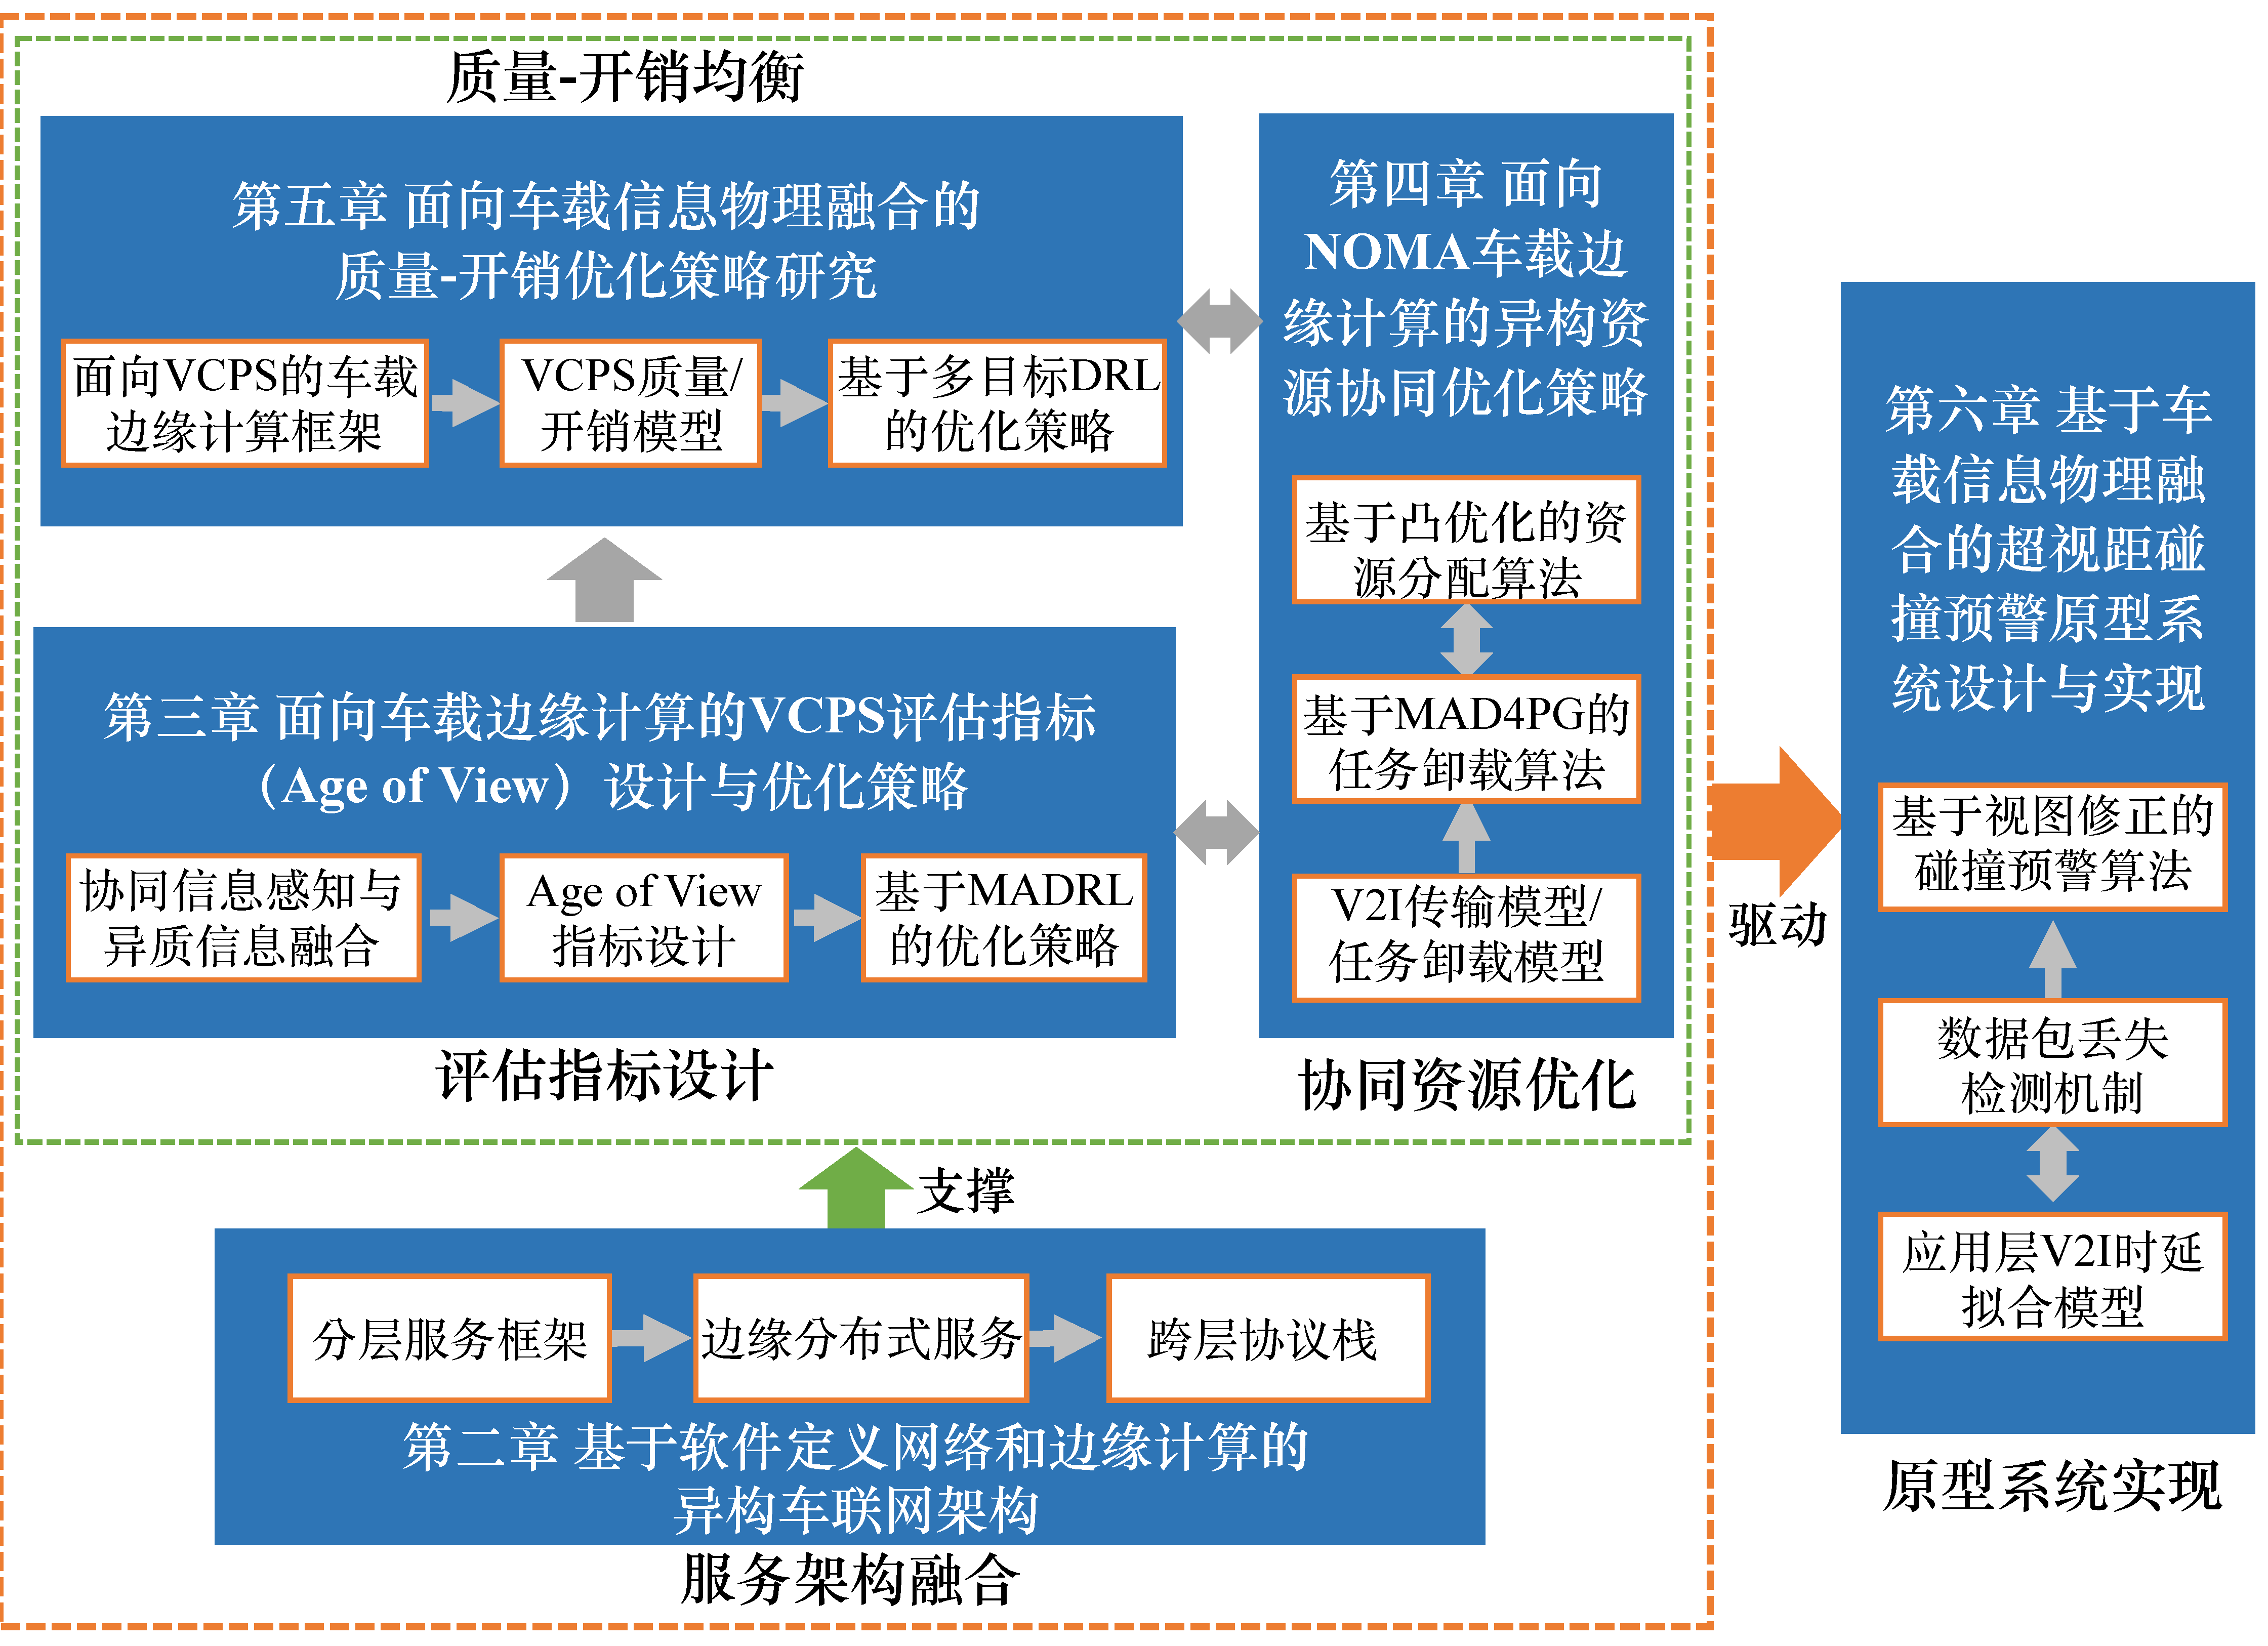
\includegraphics[width=1\columnwidth]{Fig1-4-content.pdf}
	\bicaption[主要研究内容及关系]{主要研究内容及关系}[Main research content and relationship]{Main research content and relationship}
	\label{fig 1-4}
\end{figure}

\circled{1} 基于分层车联网架构的车载信息物理融合质量指标设计与优化。
考虑车联网环境中的网络资源的高异构性、车联网物理环境分布式时变性、拓扑结构的高动态性,以及车辆节点感知能力差异性等关键特征,本文将研究融合软件定义网络和移动边缘计算的分层车联网服务架构。进一步,本文将重点研究基于分层服务架构的分布式感知与多源信息融合模型,考虑信息的多维需求,研究车载信息物理融合质量指标设计。在此基础上,研究基于差分奖励的多智能体强化学习(Multi-Agent Difference-Reward-based Deep Reinforcement Learning, MADR)算法的边缘视图优化策略。

\circled{2} 面向车载信息物理融合的通信与计算资源协同优化。
考虑车联网高动态环境与高异构分布式资源,本文将引入NOMA技术提升车联网频谱资源利用效率,并提出基于边缘协同的异构资源优化策略。本文将重点研究 V2I 传输与任务卸载模型,并在此基础上,研究基于博弈理论的多智能体深度强化学习(Multi-Agent Game-Theoretic Deep Reinforcement Learning, MAGT)算法的异构资源协同优化策略,研究基于凸优化理论的通信资源最优分配策略,并研究任务卸载势博弈模型的纳什均衡策略。

\circled{3} 面向车载信息物理融合的质量-开销均衡优化。
考虑智能交通系统中多元应用需求,本文将研究车联网中不同交通要素的视图质量与开销模型,并提出车载信息物理融合质量-开销均衡优化策略。本文将综合考虑视图的建模质量,包括信息的及时性与一致性,研究车载信息物理融合质量模型,并考虑视图的构建开销,包括信息冗余度、感知开销与传输开销,研究车载信息物理融合开销模型。在此基础上,研究基于多目标的多智能体深度强化学习(Multi-Agent Multi-Objective Deep Reinforcement Learning, MAMO)算法的车载信息物理融合质量-开销均衡优化策略。

\circled{4} 超视距碰撞预警原型系统设计与实现。
考虑动态复杂车联网环境,本文将研究基于车载信息物理融合系统的超视距碰撞预警原型系统设计与实现。具体地,本文将研究C-V2X应用层时延拟合模型和数据丢包检测机制,并研究基于车载信息物理融合系统优化的碰撞预警(Vehicular Cyber-Physical System Optimization based Collision Warning, VOCW)算法。在此基础上,研究基于 C-V2X 通信设备的硬件在环试验平台搭建方案,并研究在真实车联网环境中基于车载信息物理融合的超视距碰撞预警原型系统实现方案。

\section{论文的特色与创新之处}\label{section 1-6}

区别于目前仅专注于车联网通信协议、服务架构、资源分配和智能应用等方面的研究,本文旨在从实际需求出发,分析当前面临的挑战,并在车载信息物理融合系统的四个方面进行深入研究:架构基础与驱动核心、技术支撑、理论保障与验证手段。本文的具体特色在于:
a) 针对车联网高动态物理环境和信息感知的时效性与准确性需求,考虑到感知信息时变性、车辆节点移动性和感知能力差异性所带来的挑战,研究如何将基于SDN的集中控制和基于移动边缘计算的分布式调度有机结合,并在边缘侧建立有效的逻辑视图,为车载信息物理融合系统提供架构基础和驱动核心。
b) 针对车联网分布式异构节点资源,考虑节点异构资源的动态性、分布性和无线通信中边缘内和边缘间干扰所带来的挑战,研究如何实现边缘协同,最大化异构资源利用效率,为车载信息物理融合系统提供技术支撑。
c) 针对智能交通系统多元应用需求,考虑到车联网中不同交通要素视图质量和开销需求差异所带来的挑战,研究如何实现车载信息物理融合系统的质量-开销均衡,为车载信息物理融合系统提供理论保障。
d) 针对动态复杂车联网环境,考虑基于真实C-V2X通信设备部署和实现原型系统所带来的挑战,研究基于车载信息物理融合的超视距碰撞预警系统的原型设计和实现,为车载信息物理融合系统提供系统验证。
本文的主要创新点概述如下:

\circled{1} 提出融合软件定义网络与移动边缘计算的车联网分层服务架构,并定义边缘视图概念,率先设计视图评估指标并建立视图质量评估模型,提出分布式信息感知与多源信息融合的边缘视图构建机制:现有车联网服务架构相关研究主要关注于单一范式的实践应用,并不适用于具有大规模数据服务需求的下一代车联网场景,无法支撑车载信息物理融合系统等新兴智能交通系统应用。同时,现有研究重点关注于针对单一类型的时态数据建模与调度,难以面向车载信息物理融合系统形成有效的数据支撑。因此,本文首先综合考虑高移动数据节点、高动态网络拓扑、高异构通信资源、高分布式系统环境等车联网特征,设计基于 SDN 集中控制与基于 MEC 分布式服务有机结合的异构车联网架构。在此基础上,综合考虑感知信息的时效性、完整性与一致性,定义车联网边缘视图概念,建立针对视图质量的量化评估模型,并提出基于差分奖励的多智能体强化学习的边缘视图优化策略,实现车载边缘计算环境下的有效信息物理融合。

\circled{2} 提出基于边缘协同的异构资源协同优化策略,打破传统的单一资源优化模式:现有面向车联网资源优化策略的研究主要集中于单一资源(如通信、计算)的优化,难以满足车联网节点在不同任务中对异构资源的需求。因此,本文首先针对协同资源优化问题进行分解为任务卸载与通信资源分配两个子问题。进一步,提出基于博弈理论的多智能体深度强化学习的协同资源优化策略。具体地,将任务卸载子问题建模为势博弈模型,并证明其具有纳什均衡存在性与收敛性。最后,针对任务卸载博弈,提出基于多智能体深度强化学习的任务卸载策略。对于通信资源分配,提出基于凸优化的通信资源分配策略,实现最大化异构资源利用效率。

\circled{3} 定义车载信息物理融合系统质量与开销模型,提出基于多目标强化学习的优化策略,该策略注重实现 VCPS 质量最大化的同时同时满足 VCPS 开销最小化的要求:现有研究主要关注于基于车载信息物理融合系统的应用,而忽略了车载信息物理融合的质量与开销。因此,本文首先面向多元智能交通系统应用的差异性需求,针对车联网中不同要素建立视图模型。进一步,提出面向车联网中不同实体要素视图的质量/开销模型。最后,提出基于多目标多智能体深度强化学习的车载信息物理融合系统质量-开销均衡优化策略,以实现高质量、低成本和可扩展的车载信息物理融合。

\circled{4} 设计并实现面向车载信息物理融合的超视距碰撞预警原型系统,并在真实车联网环境下验证所提算法与系统模型:现有研究主要关注于基于仿真平台的实验验证,难以满足基于车载信息物理融合的实际 ITS 应用在真实车联网环境下的验证需求。因此,本文首先建立基于C-V2X的无线传输时延拟合模型。进一步,提出数据包丢失检测机制,并设计基于车载信息物理融合系统优化的碰撞预警算法。最后,搭建基于C-V2X设备的硬件在环试验平台,并在真实车联网环境中实现超视距碰撞预警系统原型,验证车载信息物理融合的可行性和有效性。

\section{论文的组织结构}\label{section 1-7}
本文围绕车载信息物理融合系统相关问题展开了研究。
具体地,本文将结合车联网高异构、高动态、分布式特征与智能交通系统多元需求,从车联网的架构融合与指标设计、资源协同优化、质量-开销均衡,以及原型系统实现方面进行理论研究与技术创新。
本文共分为六个章节,详细内容安排如下:

第一章,绪论。首先,介绍了车载信息物理融合系统的研究背景和国内外相关研究现状。其次,阐述了本文的研究目标与详细内容。最后,总结了本文的组织结构。

第二章,基于分层车联网架构的车载信息物理融合质量指标设计与优化。首先,设计了融合软件定义网络和移动边缘计算的分层服务架构,并提出了分布式感知与多源信息融合场景。在此基础上,设计了 Age of View 指标, 并形式化定义了车载信息物理融合质量最大化问题。其次,提出了基于差分奖励的多智能体深度强化学习的视图质量优化策略。最后,构建了实验仿真模型并验证了所提指标与算法的优越性。本章相关研究已经发表在2019年 IEEE Communications Magazine(中科院 SCI 1区),并已经投稿于 IEEE Transactions on Intelligent Transportation Systems(中科院 SCI 1区)。

第三章,面向车载信息物理融合的通信与计算资源协同优化。首先,提出了协同通信与计算卸载场景。其次,建立了V2I传输模型和任务卸载模型,在此基础上,形式化定义了协同资源优化问题。再次,提出了基于博弈理论的多智能体强化学习的资源优化策略。最后,建立了实验仿真模型并验证了所提算法的优越性。本章相关研究已经发表在2021年电子学报(CCF T1类)和2023年 Journal of Systems Architecture(中科院 SCI 2区)。

第四章,面向车载信息物理融合的质量-开销均衡优化。首先,提出了协同感知与V2I上传场景。其次,建立了VCPS系统质量和系统开销模型,在此基础上,形式化定义了最大化系统质量与最小化系统开销的双目标优化问题。再次,提出了基于多目标的多智能体深度强化学习的质量-开销均衡策略。最后,构建了实验仿真模型并验证了所提算法的优越性。本章相关研究已经投稿于 IEEE Transactions on Consumer Electronics(中科院 SCI 2区)。

第五章,超视距碰撞预警原型系统设计及实现。首先,提出了超视距碰撞预警场景。其次,设计了基于视图修正的车辆碰撞预警算法。再次,搭建了基于 C-V2X 设备的硬件在环试验平台。最后,在真实车联网环境中,实现了基于车载信息物理融合的超视距碰撞预警系统原型,验证了车载信息物理融合的可行性与有效性。本章相关研究已经发表在2020年 Mobile Networks and Applications(中科院SCI 3区)。

第六章,总结与展望。总结了全文研究内容,并讨论了后续研究计划。






